\subsubsection{Signal source}
Raw I/Q samples of each channel analysed within the window [10, 10.5]~s after the start recording instant.

\begin{figure}[H]
  \centering
  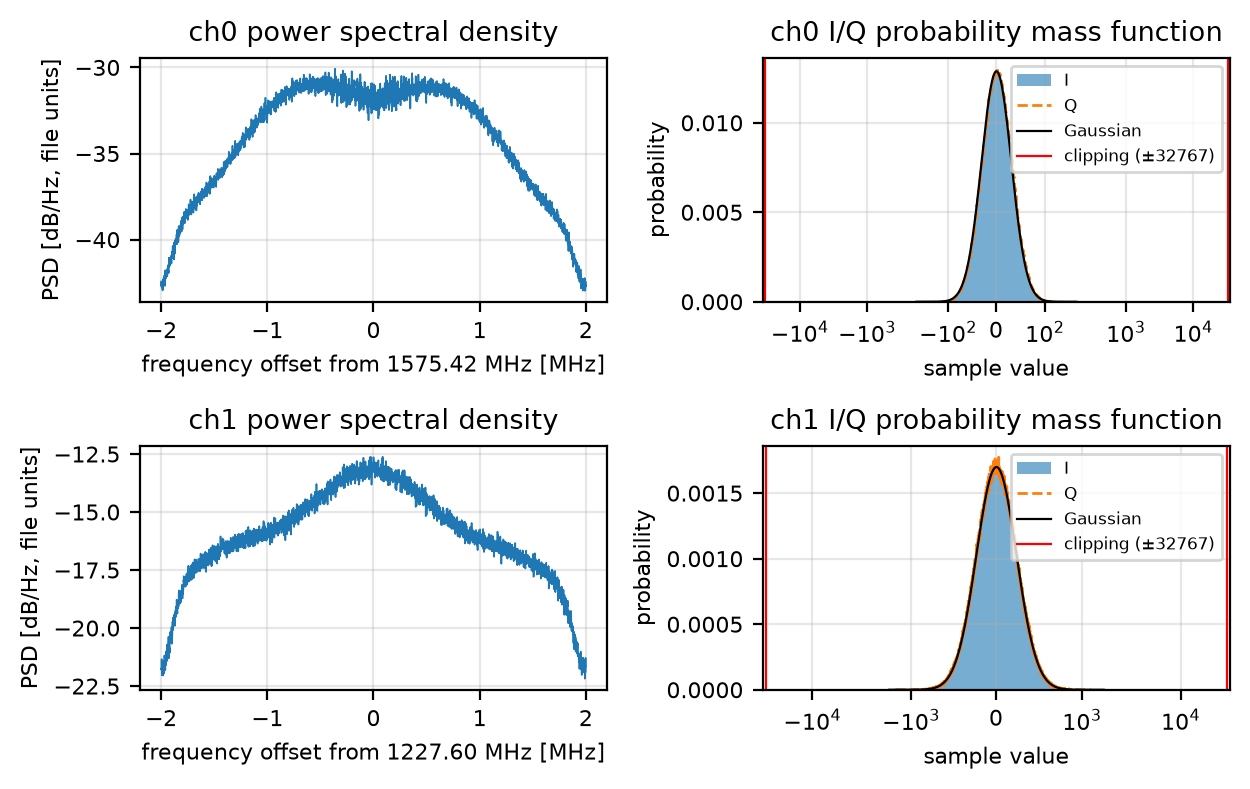
\includegraphics[width=1.0\linewidth]{gnss_sdr/l1ca16bits4msps_l2c16bits4msps_gain40/source.png}
  \caption{Signal source: power spectral density (the receiver passband over a flat thermal-noise floor; GNSS signals are below the noise, so only interference would stand out) and probability mass functions of the integer I/Q sample values (Gaussian noise, centred, not clipped).}
\end{figure}

\begin{table}[H]
  \centering
  \footnotesize
  \resizebox{\ifdim\width>\linewidth\linewidth\else\width\fi}{!}{%
  \begin{tabular}{l>{\centering\arraybackslash}p{4.2cm}>{\centering\arraybackslash}p{4.2cm}}
    \hline
    \textbf{Channel} & \textbf{ch0} & \textbf{ch1} \\
    \hline
    Frequency [MHz] & 1575.42 & 1227.60 \\
    Rate [MS/s] & 4 & 4 \\
    Format & ci16\_le & ci16\_le \\
    Bytes per complex sample & 4 (2 for I, 2 for Q) & 4 (2 for I, 2 for Q) \\
    Full scale & $\pm$32767 & $\pm$32767 \\
    Gain [dB] & 25 & 40 \\
    Std I / Q & 31.0 / 31.0 & 234.9 / 234.7 \\
    Mean I / Q & -0.01 / 0.14 & -0.73 / 0.06 \\
    Min / max I & -152 / 148 & -1211 / 1070 \\
    Min / max Q & -146 / 160 & -1202 / 1109 \\
    Headroom (full scale / std) & 1057.7 & 139.6 \\
    Clipped [\%] & 0.000 & 0.000 \\
    Lost samples & 0 & 0 \\
    \hline
  \end{tabular}}
  \caption{Signal source: sample statistics per channel (headroom: how many standard deviations of the noise fit before clipping).}
\end{table}

\subsubsection{Signal conditioner}


\begin{table}[H]
  \centering
  \footnotesize
  \resizebox{\ifdim\width>\linewidth\linewidth\else\width\fi}{!}{%
  \begin{tabular}{l>{\centering\arraybackslash}p{4.2cm}>{\centering\arraybackslash}p{4.2cm}}
    \hline
    \textbf{Channel} & \textbf{ch0 (L1 C/A)} & \textbf{ch1 (L2C)} \\
    \hline
    File format & ci16\_le & ci16\_le \\
    Source item type & ishort & ishort \\
    Data type adapter & Ishort\_To\_Complex & Ishort\_To\_Complex \\
    Input filter & Pass\_Through & Pass\_Through \\
    Resampling & Pass\_Through & Pass\_Through \\
    Rate [MS/s] & 4 $\to$ 4 & 4 $\to$ 4 \\
    \hline
  \end{tabular}}
  \caption{Signal conditioner: recorded format and rate to gnss-sdr's internal \texttt{gr\_complex} stream; both bands are read in lockstep by one \texttt{Multichannel\_File\_Signal\_Source}.}
\end{table}

\subsubsection{Acquisition}
Two-dimensional search over code delay and Doppler (one channel per band dumped; the others behave alike).

\begin{figure}[H]
  \centering
  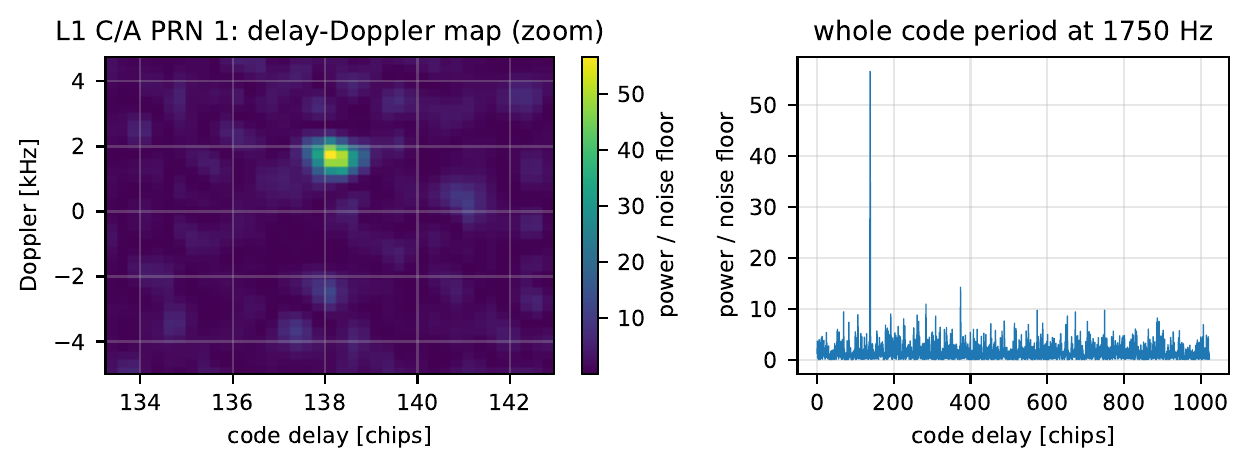
\includegraphics[width=1.0\linewidth]{gnss_sdr/l1ca16bits4msps_l2c16bits4msps_gain40/acq_1C.png}
  \caption{Acquisition, L1 C/A: delay--Doppler search of PRN 1; one sharp peak (test statistic 80 vs threshold 44) at 1750~Hz and 138.1~chips.}
\end{figure}

\begin{table}[H]
  \centering
  \footnotesize
  \resizebox{\ifdim\width>\linewidth\linewidth\else\width\fi}{!}{%
  \begin{tabular}{lrrrr}
    \hline
    \textbf{Band} & \textbf{Attempts} & \textbf{Detections} & \textbf{Detected PRNs} & \textbf{Best statistic / threshold} \\
    \hline
    L1 C/A & 1 & 1 & 1 & 1.8 \\
    L2C & \multicolumn{4}{l}{not dumped (search grid too large); acquired satellites: see the tracking table} \\
    \hline
  \end{tabular}}
  \caption{Acquisition: search attempts of the dumped channel. Attempts on satellites that are not in view (or, for L5/L2C, do not broadcast that signal) are rejected below the threshold.}
\end{table}

\subsubsection{Tracking}


\begin{figure}[H]
  \centering
  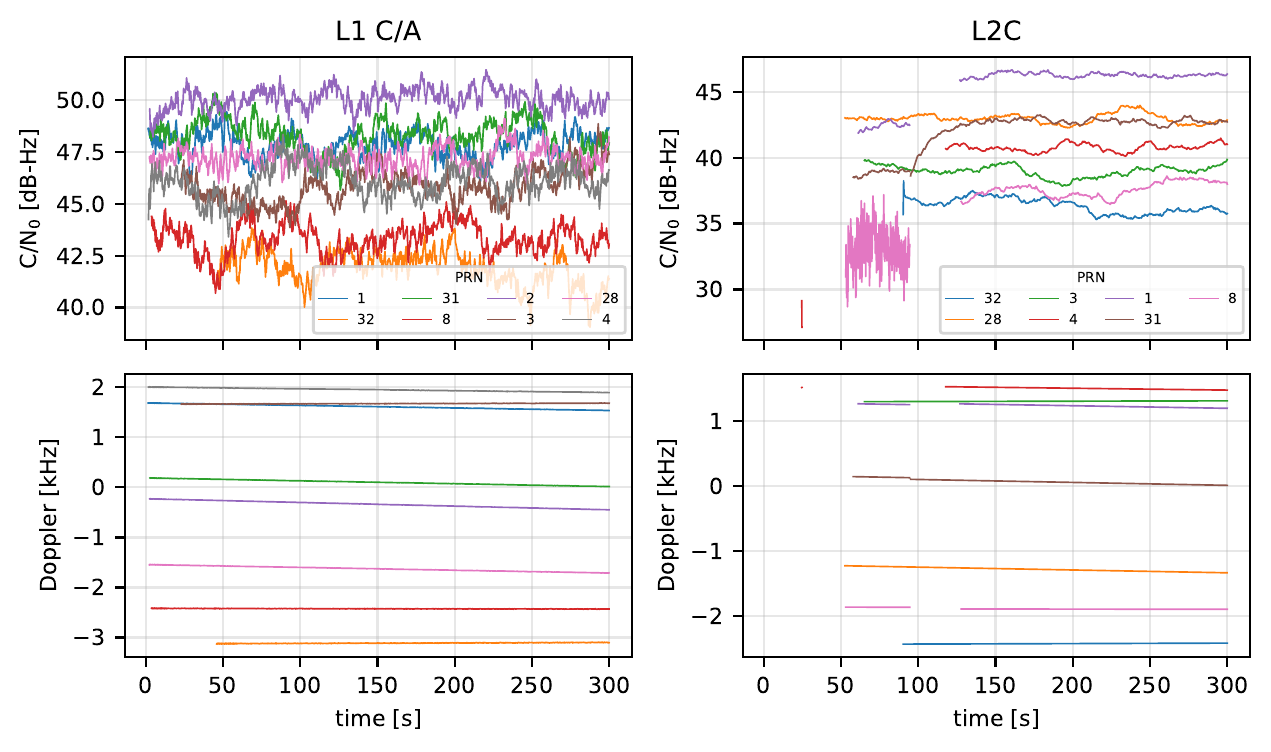
\includegraphics[width=1.0\linewidth]{gnss_sdr/l1ca16bits4msps_l2c16bits4msps_gain40/tracking.png}
  \caption{Tracking: carrier-to-noise density ratio and carrier Doppler per satellite, while phase-locked (smooth Doppler curves = loops following the real satellite motion).}
\end{figure}

\begin{figure}[H]
  \centering
  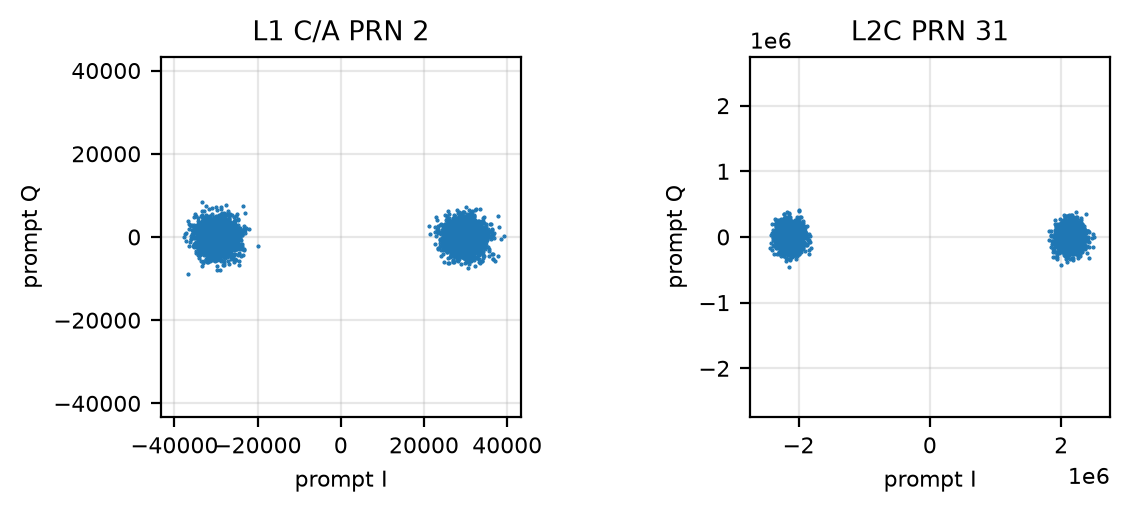
\includegraphics[width=1.0\linewidth]{gnss_sdr/l1ca16bits4msps_l2c16bits4msps_gain40/tracking_iq.png}
  \caption{Tracking: prompt correlator outputs of the strongest satellite per band. Two tight clusters on one axis (the $\pm1$ data bits; GNSS-SDR's L5 tracking puts the data component on the Q axis) mean the PLL is phase-locked; a ring would mean it is not. \texttt{Prompt\_I}/\texttt{Prompt\_Q} are 32-bit floats (sums of the samples over one integration period, in file units): they never clip, only overflowing beyond $\pm 3.4\times10^{38}$, far above the $N\cdot\text{full scale}\cdot\sqrt{2}$ a sum of $N$ samples can reach.}
\end{figure}

\begin{table}[H]
  \centering
  \footnotesize
  \resizebox{\ifdim\width>\linewidth\linewidth\else\width\fi}{!}{%
  \begin{tabular}{lrrrrrr}
    \hline
    \textbf{Band} & \textbf{Ch.} & \textbf{PRN} & \textbf{Median C/N$_0$ [dB-Hz]} & \textbf{Phase-locked [\%]} & \textbf{Losses of lock} & \textbf{Tracked [s]} \\
    \hline
    L1 C/A & 0 & 1 & 48.0 & 95 & 0 & 558 \\
    L1 C/A & 1 & 26 & 41.8 & 96 & 0 & 541 \\
    L1 C/A & 2 & 31 & 48.4 & 96 & 0 & 520 \\
    L1 C/A & 3 & 8 & 43.4 & 93 & 0 & 506 \\
    L1 C/A & 4 & 2 & 49.6 & 96 & 0 & 518 \\
    L1 C/A & 5 & 3 & 46.1 & 94 & 0 & 517 \\
    L1 C/A & 6 & 28 & 47.1 & 95 & 0 & 529 \\
    L1 C/A & 7 & 4 & 46.2 & 100 & 0 & 516 \\
    L2C & 8 & 1 & 42.7 & 70 & 2 & 274 \\
    L2C & 9 & 31 & 42.7 & 90 & 0 & 274 \\
    L2C & 10 & 8 & 33.6 & 42 & 3 & 273 \\
    L2C & 11 & 4 & 40.7 & 91 & 0 & 273 \\
    L2C & 12 & 3 & 35.3 & 20 & 4 & 273 \\
    L2C & 13 & 26 & 34.5 & 86 & 0 & 265 \\
    L2C & 14 & 28 & 41.4 & 19 & 3 & 273 \\
    \hline
  \end{tabular}}
  \caption{Tracking: per channel and satellite (phase-locked: carrier lock test $> 0.8$).}
\end{table}

\subsubsection{Telemetry decoder}


\begin{figure}[H]
  \centering
  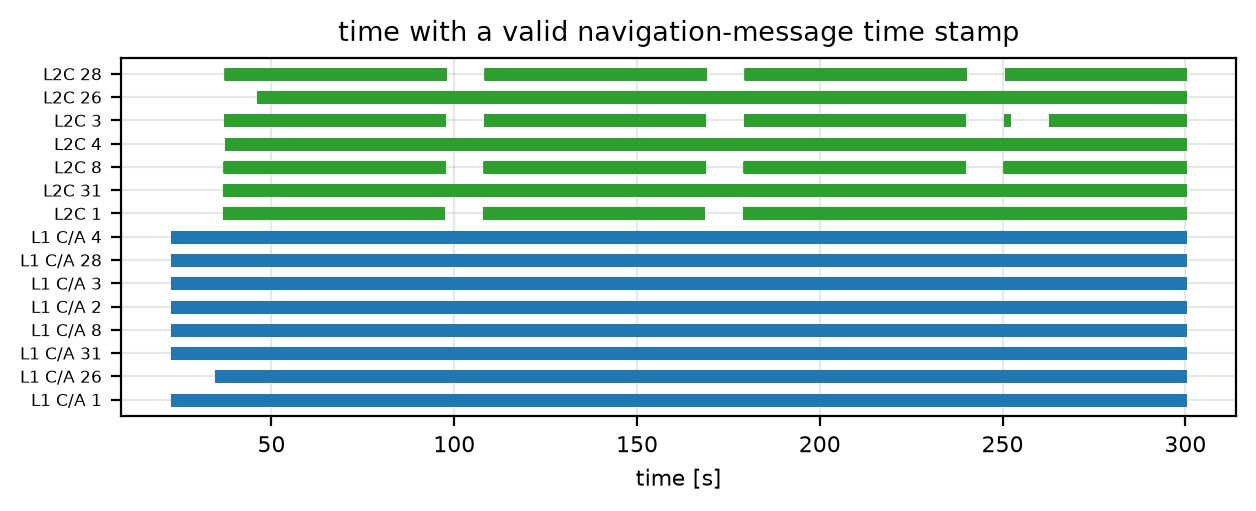
\includegraphics[width=1.0\linewidth]{gnss_sdr/l1ca16bits4msps_l2c16bits4msps_gain40/telemetry.png}
  \caption{Telemetry decoder: per band and satellite, when the decoder delivered a valid transmit time (the first one comes after the first complete frame/message).}
\end{figure}

\begin{table}[H]
  \centering
  \footnotesize
  \resizebox{\ifdim\width>\linewidth\linewidth\else\width\fi}{!}{%
  \begin{tabular}{lrrrrr}
    \hline
    \textbf{Band} & \textbf{PRN} & \textbf{Messages decoded} & \textbf{Ephemeris} & \textbf{First valid at [s]} & \textbf{TOW [s]} \\
    \hline
    L1 C/A & 1 & 46 & yes & 22.8 & 337692.0 \\
    L1 C/A & 2 & 46 & yes & 22.8 & 337692.0 \\
    L1 C/A & 3 & 45 & yes & 22.8 & 337692.0 \\
    L1 C/A & 4 & 43 & yes & 22.8 & 337692.0 \\
    L1 C/A & 8 & 47 & yes & 22.8 & 337692.0 \\
    L1 C/A & 26 & 45 & yes & 34.8 & 337704.0 \\
    L1 C/A & 28 & 43 & yes & 22.8 & 337692.0 \\
    L1 C/A & 31 & 47 & yes & 22.8 & 337692.0 \\
    L2C & 1 & 6 & yes & 37.0 & 0.0 \\
    L2C & 3 & 1 & no & 37.3 & 0.0 \\
    L2C & 4 & 15 & yes & 37.6 & 0.0 \\
    L2C & 8 & 2 & yes & 37.1 & 0.0 \\
    L2C & 26 & 12 & yes & 46.4 & 0.0 \\
    L2C & 28 & 1 & no & 37.4 & 0.0 \\
    L2C & 31 & 12 & yes & 37.1 & 0.0 \\
    \hline
  \end{tabular}}
  \caption{Telemetry decoder: L1 C/A LNAV subframes and L2C/L5 CNAV messages decoded, ephemeris obtained, and the first valid time of week.}
\end{table}

\subsubsection{Observables}
Pseudorange, carrier phase and Doppler of every channel at common receiver epochs.

\begin{figure}[H]
  \centering
  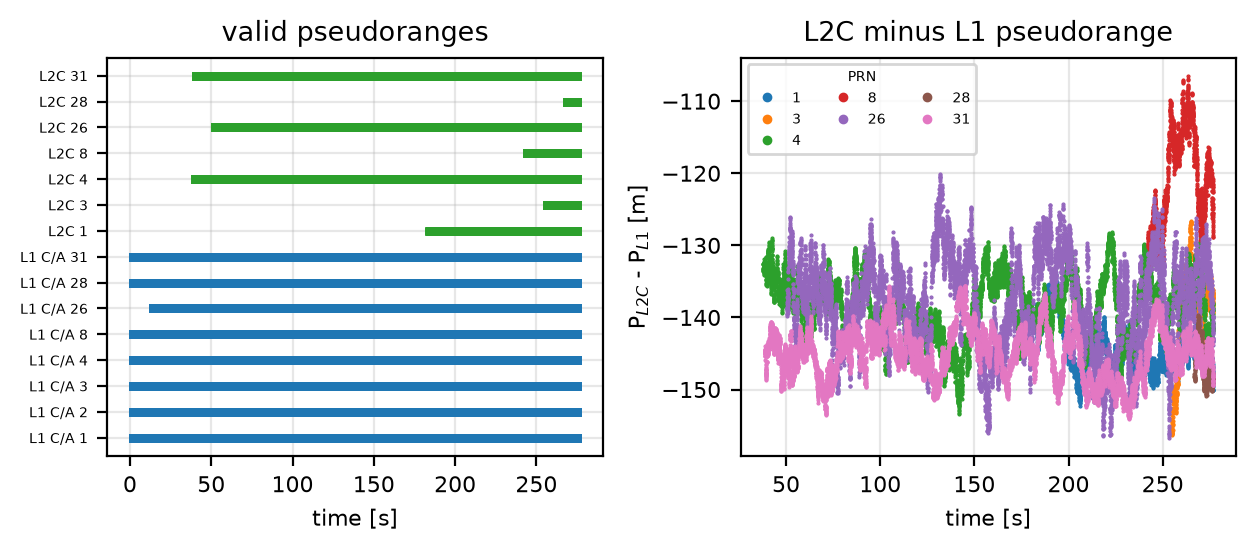
\includegraphics[width=1.0\linewidth]{gnss_sdr/l1ca16bits4msps_l2c16bits4msps_gain40/observables.png}
  \caption{Observables: epochs with a valid pseudorange per band and satellite, and the difference between the two bands' pseudoranges of the same satellite (a constant receiver inter-band bias, the same for every satellite, plus the slowly varying ionospheric delay).}
\end{figure}

\begin{table}[H]
  \centering
  \footnotesize
  \resizebox{\ifdim\width>\linewidth\linewidth\else\width\fi}{!}{%
  \begin{tabular}{lrrrrr}
    \hline
    \textbf{PRN} & \textbf{Common epochs} & \textbf{of run [\%]} & \textbf{Mean [m]} & \textbf{Std [m]} & \textbf{Drift [m/s]} \\
    \hline
    1 & 4732 & 32 & -144.35 & 3.13 & -0.0455 \\
    3 & 1110 & 7 & -138.97 & 6.09 & 0.4556 \\
    4 & 11956 & 80 & -138.55 & 4.09 & 0.0006 \\
    8 & 1740 & 12 & -120.53 & 6.57 & 0.2375 \\
    26 & 11324 & 76 & -137.94 & 6.31 & -0.0046 \\
    28 & 508 & 3 & -146.62 & 2.76 & -0.6129 \\
    31 & 11918 & 80 & -145.04 & 3.36 & -0.0058 \\
    \hline
  \end{tabular}}
  \caption{Observables: P$_{\mathrm{L2C}}$ $-$ P$_{\mathrm{L1}}$ per satellite at common epochs (similar means = shared receiver bias; std = code noise of both bands).}
\end{table}

\subsubsection{PVT}
Position from the pseudoranges and the decoded ephemeris, compared with the surveyed antenna position (-23.209433$^\circ$, -45.874875$^\circ$, 596.42~m).

\begin{figure}[H]
  \centering
  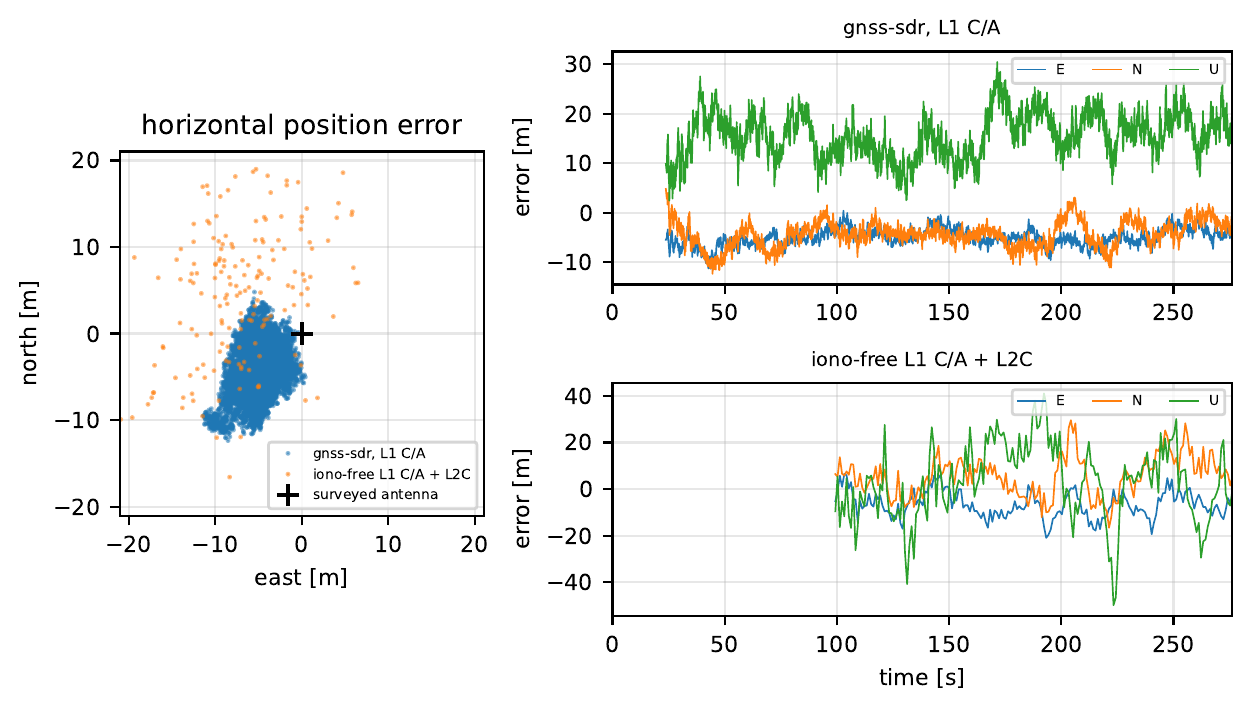
\includegraphics[width=1.0\linewidth]{gnss_sdr/l1ca16bits4msps_l2c16bits4msps_gain40/pvt.png}
  \caption{PVT: position error with respect to the surveyed antenna position. L1 C/A: gnss-sdr's own solution (broadcast ionosphere model). Iono-free: computed from gnss-sdr's observables and decoded ephemeris (gnss\_spp.py), removing the ionospheric delay with the second band (pseudoranges carrier-smoothed over 100~s).}
\end{figure}

\begin{figure}[H]
  \centering
  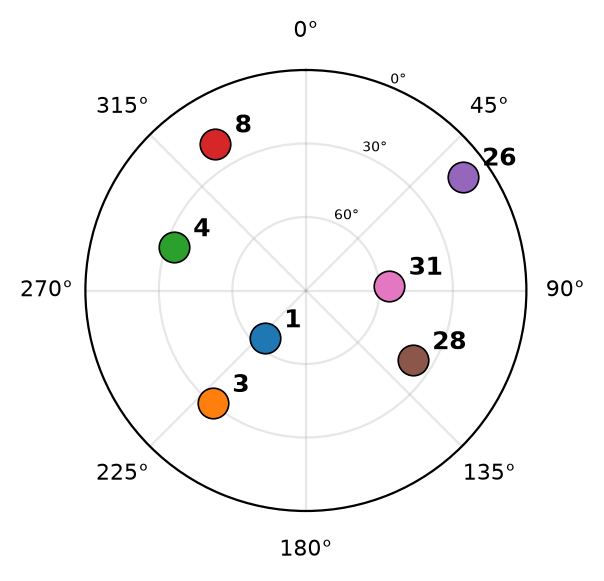
\includegraphics[width=0.45\linewidth]{gnss_sdr/l1ca16bits4msps_l2c16bits4msps_gain40/skyplot.png}
  \caption{PVT: sky plot of the satellites in the dual-frequency solution (azimuth, elevation) during the recording.}
\end{figure}

\begin{table}[H]
  \centering
  \footnotesize
  \resizebox{\ifdim\width>\linewidth\linewidth\else\width\fi}{!}{%
  \begin{tabular}{l>{\centering\arraybackslash}p{4.2cm}>{\centering\arraybackslash}p{4.2cm}}
    \hline
    \textbf{Solution} & \textbf{gnss-sdr, L1 C/A} & \textbf{iono-free L1 C/A + L2C} \\
    \hline
    Solutions & 13149 & 35 \\
    Run with fix [\%] & 92 & 13 \\
    Mean E / N / U [m] & -5.0 / -4.5 / 15.5 & -6.4 / 17.2 / 14.0 \\
    Std E / N / U [m] & 1.7 / 2.6 / 4.7 & 5.4 / 14.6 / 29.9 \\
    RMS 2-D [m] & 7.4 & 24.1 \\
    RMS 3-D [m] & 17.8 & 40.9 \\
    95\% horiz. [m] & 11.1 & 45.4 \\
    \hline
  \end{tabular}}
  \caption{PVT: position error statistics with respect to the surveyed antenna (mean = accuracy, std = precision; \% of the run's seconds with a position; gnss-sdr outputs several solutions per second, the iono-free one is computed once per second).}
\end{table}

